%!TEX root = foo-thesis.tex

\chapter{Concept}

\section{Lighting Pipeline Overview}

\begin{figure}[h]
    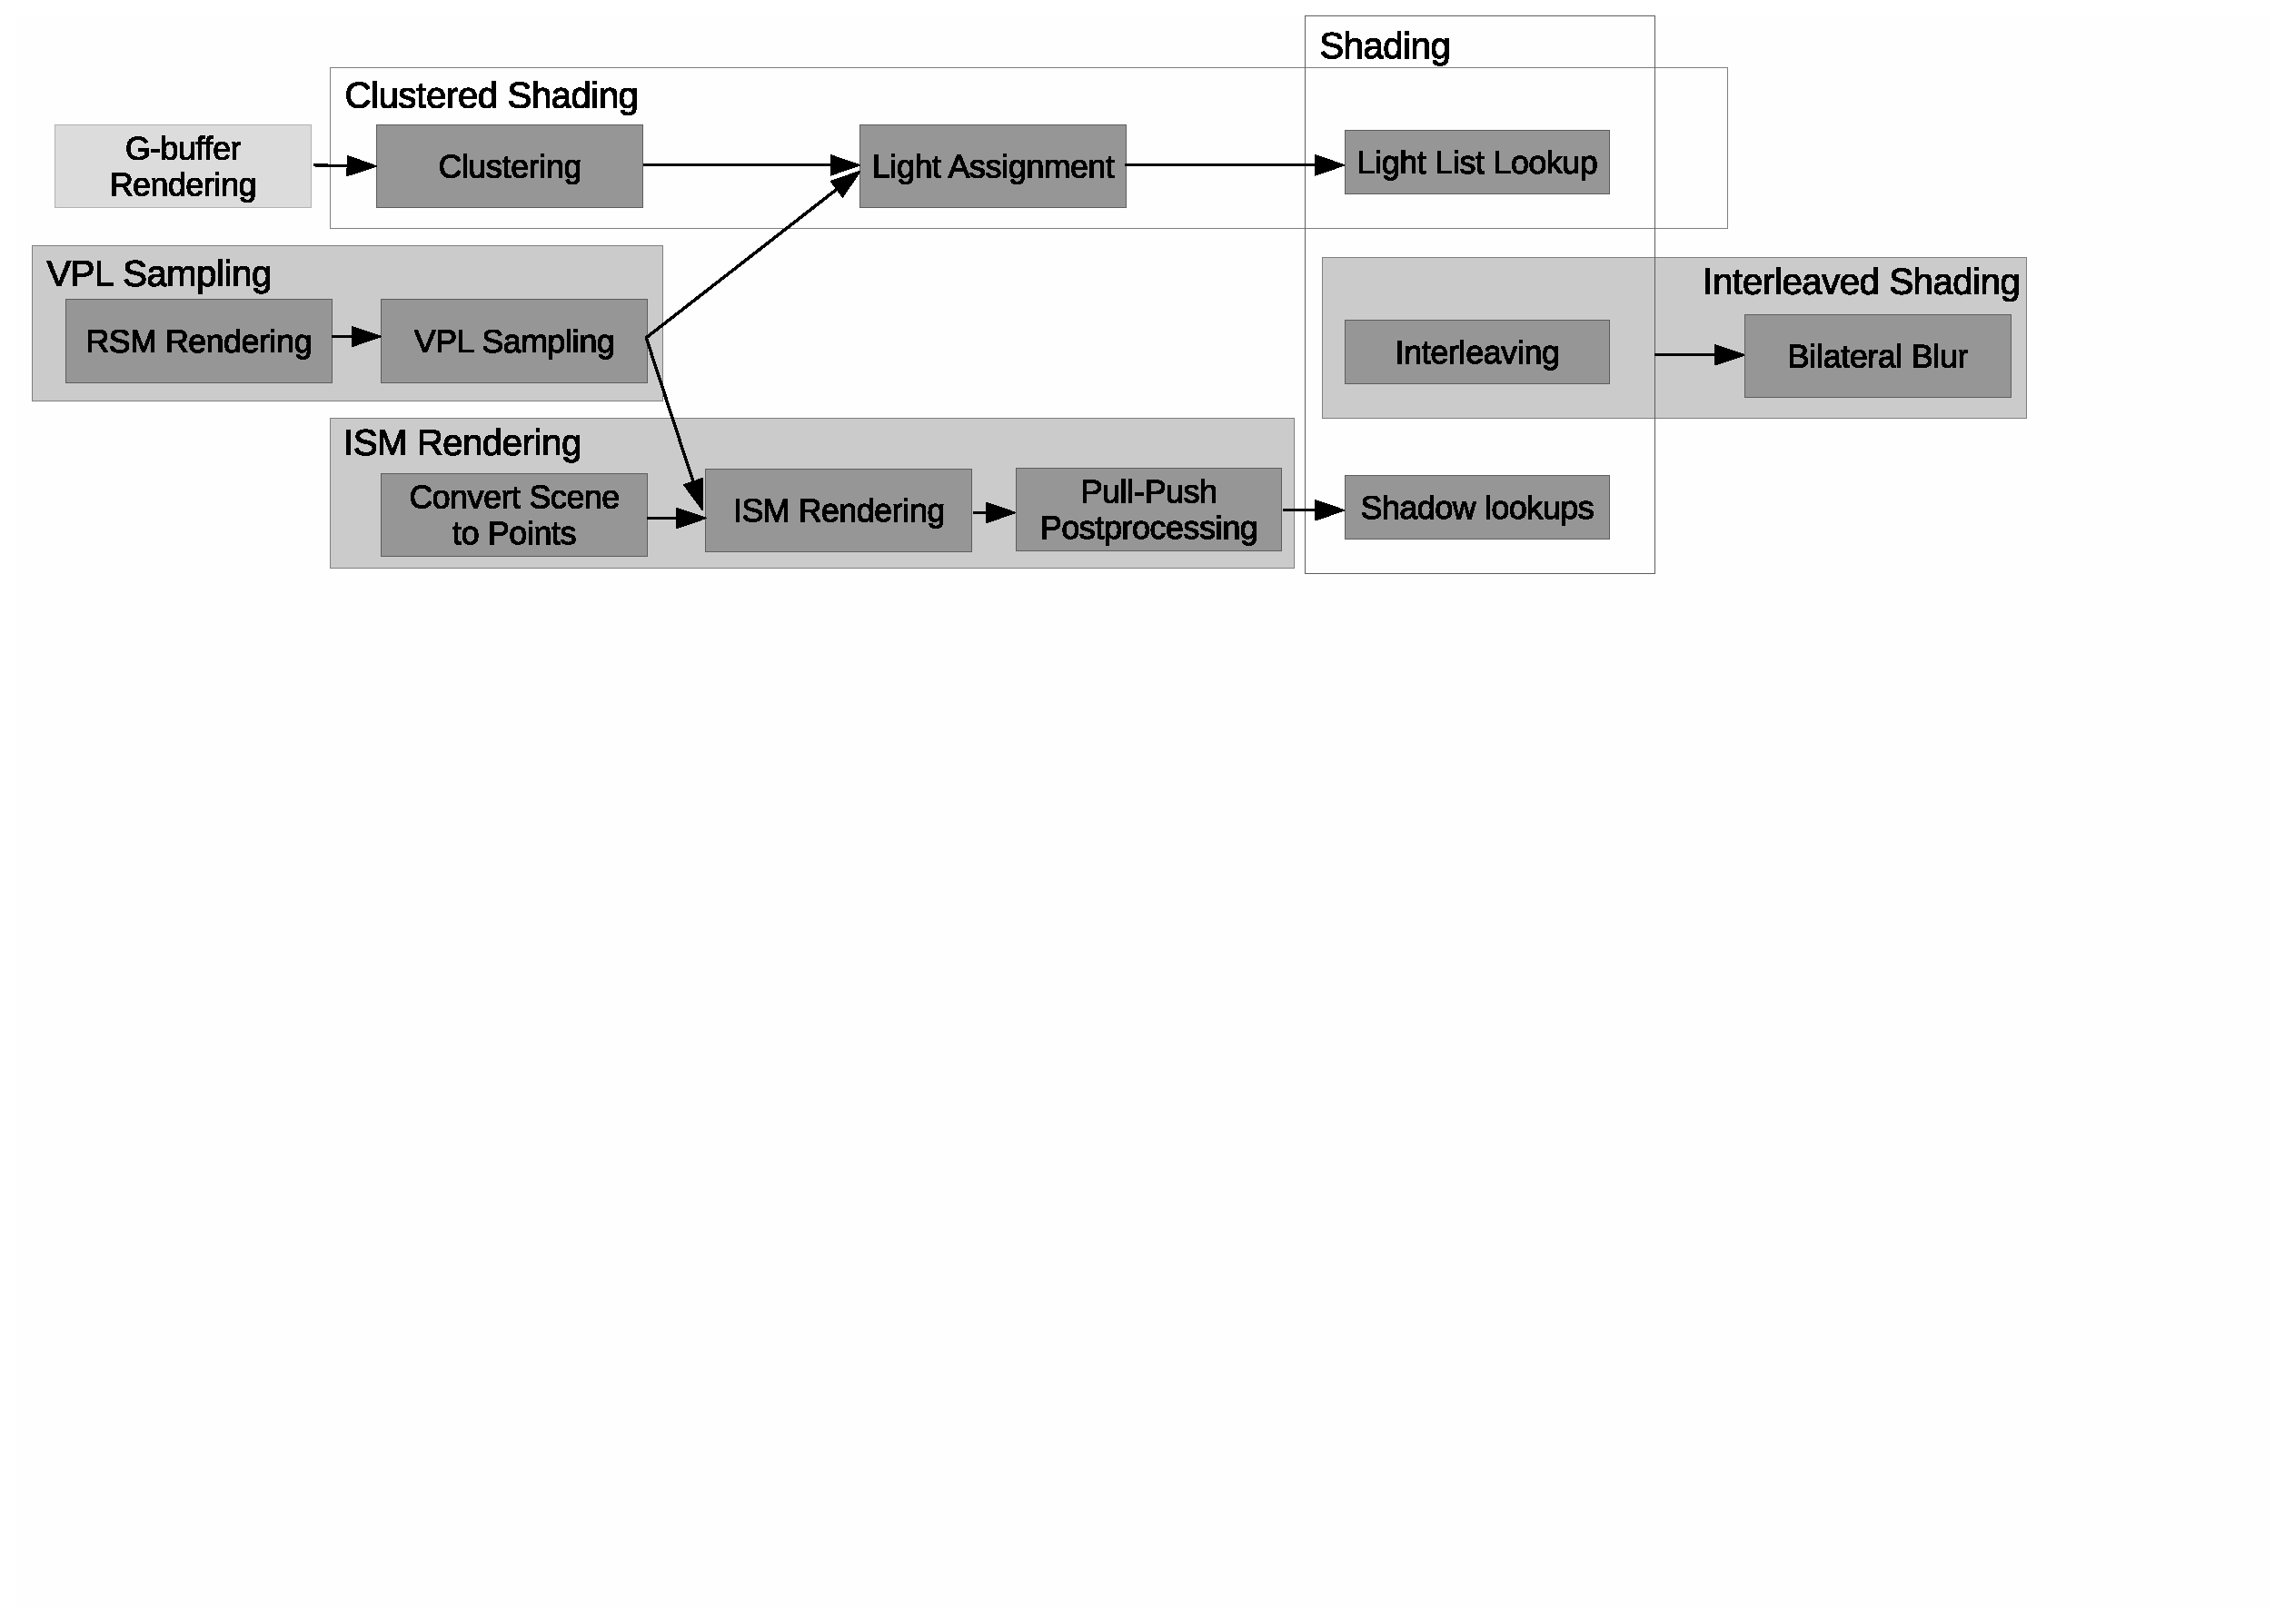
\includegraphics[width=\textwidth]{graphics/Lighting_pipeline_concept_rough}
    \caption{Lighting pipeline concept.}
    \label{fig:LightingPipelineConcept}
\end{figure}

\todo{bilateral blur into that diagram?}

\todo{do the matrix the other way around?}

\todo[color=orange]{Indirect shading? indirect illumination? just shading?}

This chapter will detail the individual stages of the lighting pipeline presented in this thesis. Figure~\ref{fig:LightingPipelineConcept} provides an overview.
Our G-buffer rendering does not differ from common deferred rendering pipelines and is not covered further.
The reflective shadow map and the subsequent VPL sampling will be covered in the following section.
Section~\ref{sec:ISM} describes the rendering process for the imperfect shadow maps in detail.
The shading, which uses interleaving and the clustered deferred technique, is explained in Section~\ref{sec:interleavedAndClusteredShading}.
Finally, we use clamping to remove singularities, this is shortly presented in Section~\ref{sec:clamping}.


\section{Virtual Point Light Sampling with Reflective Shadow Maps}
\label{sec:RsmVplSampling}

VPL sampling has not been the focus of this thesis, therefore we use a rather basic approach by rendering a  reflective shadow map \parencite{Dachsbacher:2005:RSM} and regularly sampling it. \citet{hedman2016sequential} present a more advanced approach.

\begin{outline}
\1 Often preferred due to the simplicity and speed because rasterization. but, first bounce only.

\1 Similar to regular G-Buffer rendering

\1 Like shadowmaps, scene is rendered from the light's viewpoint

\1 Unlike shadowmaps, not only depth is rendered but additionally normal and (diffuse) surface color.

\1 The result can be sampled to create VPLs with a certain position reconstructed from the depth buffer, and normal and color taken from the additional buffers.

\1 In our case, we use regular sampling. Importance-based approaches are available, also the samples can be clustered \cite{} or chosen relative to their estimated contribution to the final output. \citet{hedman2016sequential} uses a different approach without RSMs.

\end{outline}

\section{Solving Occlusion with Imperfect Shadow Maps}
\label{sec:ISM}


The original paper \citep{ritschel2008ism} converts the scene geometry to a point set in a preprocessing step and uses the points to efficiently render hundreds of shadow maps in parallel. They use splatting to render the points and fill the resulting holes in the shadowmaps with a pull-push algorithm inspired by \citep{Marroquim:2007:reconstruction}.

\citet{ritschel2011ismsViewAdaptive} build on \citet{laine2007incremental} this by converting the scene to a triangle texture dynamically, and sampling the points from that texture. Instead of computing a triangle texture, \citet{barak2013temporally} use the tessellation units of recent GPUs to dynamically convert triangles into points.
We follow this approach since it is relatively simple to implement and inherently dynamic, but have not implemented the adaptive sampling from \citet{ritschel2011ismsViewAdaptive} yet.
\citep{ritschel2008ism} also present multi-bounce indirect illumination with their technique, which we have not implemented.
We describe the point rendering process in the following section and subsequently detail the pull-push algorithm.

\subsection{Point Rendering}
\begin{outline}
\1 render the scene
\1 depending on the size of the triangle, set tessellation levels
\1 of the resulting tessellated triangles, take the center, calculate approx world size of disk, take normal from buffer
\1 while it might be faster to just use the vertices as points, we take the center of each triangle to be more accurate, otherwise the points on the edge of the triangle will enlarge the rendered area considerably.
\1 pick a random VPL, perform culling, render splat
\1 actually, we iterate over several VPLS, and collect some that pass the culling test, and render to those. more in implementation chapter
\1 mention the two approaches? single pixel vs large splats?
\1 also drop that it's a paraboloid projection
\end{outline}

\subsection{Pull-Push Postprocessing}

\begin{outline}
\1 While \citep{ritschel2008ism} implement a simplified variant of \citet{Marroquim:2007:reconstruction} and only use depth information from the point rendering, this approach trades in accuracy for performance and simplicity. We follow \citet{Marroquim:2007:reconstruction} more closely and additionally use a size attribute (and normal) for each point.

\1 rough overview: the algorithm is a ``pyramid-method''? and uses miplevels.
\1 a pull phase aggregates the information from four pixels of a finer level to one pixel of a coarser level.
\1 It only considers valid pixels, i.\,e. ???
\1 the push phase aggregates four pixels of the coarser level for each pixel of the finer level.
\1 Again only pixels that are valid, i.\,e. ???
\1 we differ from the original implementation by...
\end{outline}
\todo{expand on this}



\section{Interleaved and Clustered Deferred Shading}
\label{sec:interleavedAndClusteredShading}
\citep{Keller:2001:InterleavedSampling} is often used to vastly improve the performance impact of GI methods.

\begin{outline}
\1 general idea: given some amount of samples that, in a naïve implementation, would be performed per pixel, distribute those samples over a block of pixelssome samples per pixel in a 4x4 or 8x8 block
\1 the naïve implementation hurts cache coherency, since adjacent pixels process different samples.
\1 to this end, de-interleaving is often used to simultaneosly process those pixels that use the same sample set. see \ref{sec:impl:interleavedShading} for details.

\1 results in structured noise and missing information as all pixels have only part of the samples
\1 therefore, geometry-aware blur similar to \citet{laine2007incremental} to distribute the information

\1 all this works because low-frequency effect

\1 we use a 4x4 sampling pattern and laine's algorithm for blurring.


\1 in addition to interleaved sampling, we also employ a technique taken from \citet{olsson2012clustered}
\1 view frustum is divided into a fixed number of clusters
\1 for each fragment, determine cluster. clusters with no fragments are ignored.
\1 for each cluster, determine the VPLs that can reach that cluster, put into light list.
\1 during shading, don't iterate over all VPLs but only those from the light list.
\1 usually, large benefits due to limited radius. we have infinite radius, but at least we can discard half the lights because hemisphere.
\1 ritschel's paper about clustering

\end{outline}

\section{Removing Lighting Singularities through Clamping}
\label{sec:clamping}
It's simple, we clamp the singularities. Wouldn't be necessary with infinite number of lights. \citet{hedman2016sequential} reach high accuracy even with clamping and 2k lights.
